This chapter explains about the major tasks implemented in the thesis, new contributions made to the PUF Toolkit. The first part of the chapter briefly explains about the current PUF toolkit implementation, without delving much into the details. The second and more major part talks about the new modifications that were done to the toolkit in the form of BCH fuzzy extractor encoder and decoder integration, which were previously not a part of the main toolkit and presented as seperate executables
with seperate menu items. We then go on to explain the Golay code implementation both the decoder and encoder, and explain their integration in the toolkit as a distinct menu item. Then the other modifications like the addition of \emph{'offsets from begining and end', error codes} and other intricate code developement changes are presented together as one section.\\

TODO: write about hamming distance and jaccardi's index

The final two sections deal with cognicrypt details and the Java Native Interface (JNI), they first touch upon the basics of JNI
wrapper and the functioning of JNI with shared libraries packaged as JAR files that are accesible to Java compiler as external library. Finally, we describe the clafer model of the cognicrypt and how it assists users and Java developers, without any previous knowledge about cryptography, to select a strong PUF based secure key evaluation algorithm based on the questions asked by the cognicrypt. In the end of this last section we also talk about the xsl model of the cognicrypt that builds on
the clafer model to generate a boilerplate java code to help the Java developer by presenting him/her with a sample usecase of the Java code implementation showing a usage of the PUF evaluation algorithms that is robust and flawless.\\

For the implementation, the ISO standardize programming language C++ was chosen. This selection was made based on the efficient and general purpose features provided by C++. Apart from the object oriented and generic programming features, C++ has a high abstraction level and the compilation and code development can be done on diverse systems. The implementations are dissociated from a specific hardware to support a wide range of systems and applications. This makes the toolkit easier
to extned and conform to a particular hardware for next iterations. The JNI framework support native calls and the wrapper is written in Java, for clafer model we use Java script and json files along with the .cfr clafer extension modelling language(refer to github page [ ] for details) and xsl model to generate sample Java boilerplate code is written in xsl.\\

\section{PUF Toolkit}
The current implementation of the PUF toolkit was done and presented in the thesis [sebastian Master Thesis]. The main aim of the toolkit is to evaluate various PUF repsonse based on well established metrics and thereby helping researchers and designers to gain useful insights into the properties and behaviour of PUF responses. The toolkit implements the following list of metrics: \pagebreak

\begin{itemize}
	\item (Shannon) Entropy
	\item Hamming Weight
	\item Intra-Hamming Distance
	\item Inter-Hamming Distance
	\item Min-entropy
	\item Median and average
\end{itemize}

These metrics are well explained in the Master thesis Sebastian [ ], so we take the liberty to not go into the detail of explaining each metric here again. It must also be noted that there are other metrics and definitions that use identical concepts and/or apply the metrics in a different way to generalize the coorelation between different PUF instances and their reponses. More exhaustive and comprehensive information related to these metrics and definitions for PUFs can be found in [seb 37, 53, 26, 5].\\

Apart from the above mentioned metrics implementation the PUF based secure key storage is implemented already, using BCH encoder and Decoder in two seperate executables. The structure and the User design used in these two executables is similar to the PUF toolkit and to avoid confusion we shall refer to them as \emph{PUF-BCH encoder} and \emph{PUF-BCH decoder}.\\

\subsection{User Design}

The notion behind the console user interface design by inspired from Nielsen and Molich's nine user interface design guidelines [seb 45]. These guidelines and their resulting effects are shown the table \ref{tab:guidline_design} below:

\begin{table}[!ht]
\begin{center}
\begin{tabular}{cll}
\toprule
\multicolumn{1}{c}{\textbf{No.}} &\multicolumn{1}{c}{\textbf{Guideline}} & \multicolumn{1}{c}{\textbf{Effect}}\\
\midrule
\hline
1 & Simple and natural dialogue & Clear and logical dialogue structure\\

2 & Speak the user’s language & Clear instructions\\

3 & Minimize the user’s memory load & Clean design, brief help and guide texts\\

4 & Be consistent & Consistent design in all menus\\

5 & Provide feedback & Provide feedback and status\\

6 & Provide clearly marked exits & Provide ``back’’ and ``exit’’ in each menu\\

7 & Provide shortcuts & Inputs by abbreviations \\

8 & Good error messages & Provide useful error messages\\

9 & Prevent errors & Handle wrong inputs \\
\hline
\addlinespace
\bottomrule
\end{tabular}
\end{center}
\caption{The nine design guidelines according to [seb 45] and the effect on the UI design.}
\label{tab:guidline_design}
\end{table}

The design of the menu and the (sub-) menus is consistent and recurses itself to make the user interface more intuitive and friendly. Each menu option is written in clear and easy to understand instructions and the menu items are precisely structured to help the user navigate the toolkit with ease. The organization of the menu follows a hierarchical design and a ``back'' function is provided for the user to go to the parent menu. A conceptual depiction of the User Interface is shown in Figure
\ref{img:gui_design}. The Graphical User Interface (GUI) is subdivided into four parts, the color markers are related to the illustration in \ref{img:gui_design}:

\begin{itemize}
	\item The first part, marked in yellow, is the \emph{header}. It gives the user general information, like the title of the current (sub-) menu or brief instructions.
	\item The second part of the gui shows the options and functions that the user can choose from the (sub-) menu, the number infront must be input by the user in the last part of the GUI. The conceptual illustration for the part is marked in red and is called as \emph{Menu}.
	\item Below the Menu part there is \emph{settings and results} that are marked in blue. It shows the current configuration and provides the user with essential information that is vital for the actual computation of the main function. It also shows the output after the computation is performed in the result part of this section.
	\item The fourth part of the GUI is for \emph{feedback} and inputs and is marked in green. It presents the user with the actual processing status, or if an error occurred and the type of the error. Also, it contains a user interactive input cursor, a number must be typed in by the user in order to select the options/functions from the second part, Menu of the GUI.
\end{itemize}

\begin{figure}
\centering
\fbox{ 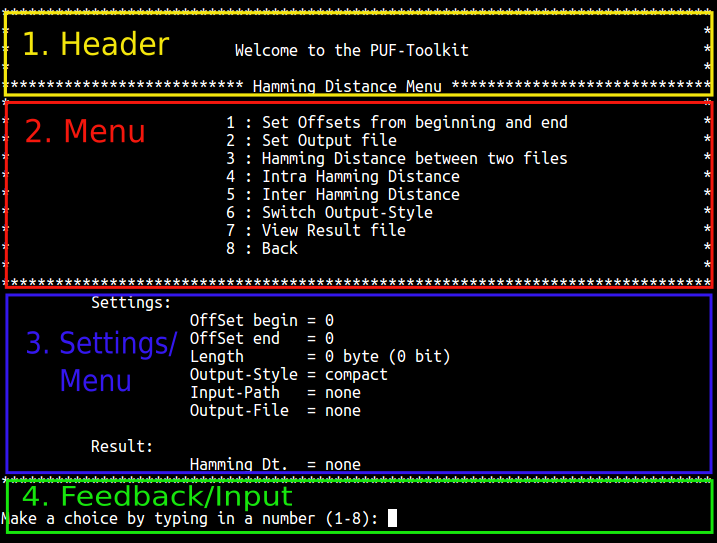
\includegraphics[width=0.9\textwidth]{images/toolkit_gui4.png}}
\caption{Conceptual design of the PUF Toolkit user interface.}
\label{img:gui_design}
\end{figure}

The design of the GUI is kept simple without the use of extended graphic components to keep the toolkit compatible with other operating systems like linux. The UI shows only relevant information depending on the current state of the program and potrays a simple but aesthetic clean design. Error correction and incorrect user input is efficiently handled, all possibile inputs are exhausted and depeding on the false input, meaningful errors information is displayed to the user, that can be used to
recover from the erroneous state. Also for all mandatory inputs a brief guide / help text with examples is shown, the current settings are saved and kept in each (sub-) menu (wherever applicable) to avoid unecessary redudant input.\\

Rigorously complying to the standardized design guidelines for the toolkit, resulted in a effective and intuitive console user interface.
This in turn decisively supports developers and researchers in the PUFs reponses evaluation.[seb thesis]

\section{Hamming Distance Menu}

The hamming distance functionality was added to and integrated as part of this Master thesis. Hamming Distance between two bit strings of same length is defined as the number of the bits that differ amongst the two binary bit strings. For eg. if we have two string \emph{A = 1100} and \emph{B = 1010} then the hamming distance between them would be ``\emph{two}'', since the bits at second and third position (starting from the left) differ between these two strings. The implementation of
this functionlality is straightforward, using the in-built \emph{bitwise XOR} operation of the ISO C++ standard and then counting the number of ones in the resulting string, which is nothing but calling the hamming distance function on the resultant string.\\

As depicted in the figure \ref{img:gui_design} above there are other options like \emph{Intra Hamming Distance} and \emph{Inter Hamming Distance} in the Hamming Distance Menu, that are organized later as subsections where we explain about the different modes and other options and plausible input values the user can select from them. For now we direct our attention at the other menu items.\\

The first menu item is related to the \emph{\textbf{Offsets}} that are mandatory for the user to input and the first query that must be answered after the toolkit is run. Since the PUF toolkit is designed for evalutation of PUF responses that are in binary format and not all the data in PUF reponse binary file is useful for evaluation the user can manually select how much he/she desires to skip the data (in bytes) from the beginning and the end of the file using this \emph{Offsets} option.
For example the first $400$ bytes of the PUF response of a (TI) Stellaris LM4F120XL Launchpad Evaluation Kit are used during the booting process and are not random, so they are irrelevant in PUF responses evaluation. These kind of device specfic behavior requires suitable handling to ensure valid results.\\

Consequently the \emph{Offset} determines the selection range of the bytes from the PUF response for calculation and also establishing the actual \emph{length} of the response. For eg. if a PUF response is 32784 bytes long and we skip 400 from the beginning and 200 from the end, the actual length becomes $32784-600 = 32184$ bytes and the processing starts from the $401^{th}$ byte till $32184^{th}$ byte.\\

The result of the Hamming Distance between two PUF responses can be optionally stored in an output file that is set using the option \emph{two}. This is not mandatory if we are evaluating only two files but in cases of Inter/Intra Hamming distance this option becomes mandatory. Another functionality added to the Hamming Distance and other Functions in the toolkit as well is that of the Fractional Distance. \newline
$\S$\emph{Defintion}: We define \emph{Fractional Hamming Distance} as the Hamming Distance between two PUF
responses divided by their length. For example if Hamming Distance between two PUF responses each of length 31784 bytes is 10, then their Fractional Hamming Distance would be $ 10 / 31784 = 0.000314624$ (NOTE: the toolkit displays the fractional hamming distance rounded off to 9 digits after decimal).\\

The Hamming Distance can be calculated using option \emph{three} that will ask for the two PUF responses binary filenames and if the path and filenames are correct, the results will be displayed in the fourth part of the GUI. If the output filename was given before then the result is also stored in that file and can be viewed using the option \emph{seven}.\\

In order to understand the code flow and working of the hamming distance function it is vital to look at the structure \emph{Item} and its data members. This structure is used by other menus in the toolkit to share the current settings and global configurations like Offsets, filenames, paths etc. and thereby reducing the user's effort and memory load. The table \ref{table:item} only highlights the data members and their purpose that are relevant to Hamming Distance Menu. The other data members
for the time being are not shown and will be discussed in relevant sections.\\

\begin{table}[!ht]
	\begin{center}
		\begin{tabular}{ll}
			\toprule
			\multicolumn{1}{c}{\textbf{struct \emph{Item}}} & \multicolumn{1}{c}{\textbf{Purpose}}\\
			\midrule
			\hline

			\emph{offset\_begin} & Defines the starting point in a binary file (bytes to skip from beginning)\\

			\emph{offset\_end} & Defines the ending point in a binary file (bytes to skip from end)\\

			\emph{input\_length} & Defines the number of bytes to use \\

			\emph{input\_file\_name} & Defines the name of the first input file (name and path)\\

			\emph{input\_PUF\_name} & Defines the name of the second input file (name and path)\\

			\emph{output\_file\_name} & Defines the name of the output result file (name and path)\\

			\emph{zeros} & Stores the occurrences of 0s in a defined file\\

			\emph{ones} & Stores the occurrences of 1s in a defined file\\

			\emph{frd} & Stores the fractional distance in a defined file\\

			\emph{result} & Stores the result and feedback regarding the calculations\\

			\emph{HD\_error\_pos} & Additional error information \\

			\hline
			\addlinespace
			\bottomrule
		\end{tabular}
	\end{center}
	\caption{Definition of the elements of the data structure \emph{Item} and their purpose.}
	\label{table:item}
\end{table}

The four lines of code form the basic building block for hamming distance as shown in the listing \ref{lst:hammingdt}. First the data is read from the two input PUF files into two arrays of size \emph{dsize} where dsize is equal to the length of the files after applying the Offsets, then as depicted in lines 3-5 of the listing \ref{lst:hammingdt} each byte of the data are bitwise XORed and the result in stored in a third array of same length. So the resultant data array contains
\emph{ones} in the position where bits differ in the two PUF responses. We then just need to count the number of ones in the XORed result.
This is done by calling the function \emph{hammingwt} abbreviated in the code for Hamming Weight.\\

\begin{center}
\begin{minipage}{0.7\textwidth}
\begin{lstlisting}[frame=single,language=C++,
commentstyle=\color{green},
backgroundcolor=\color{gray},
keywordstyle=\color{blue},
stringstyle=\color{orange},
basicstyle = \ttfamily \color{black} \footnotesize,
caption={Hamming Distance calculation using hamming weight and bitwise XOR operator} ,
label={lst:hammingdt},
captionpos=b,
numbers=left]
    //bitwise XOR f1data and f2data
    //to get the positions where bits differ
    for (i = 0; i < dsize; i++) {
        data[i] = f1data[i] ^ f2data[i];
    }
    //calculate hamming distance
    item->ones = hammingwt(data, dsize);
    item->frd = (float) item->ones / dsize;
\end{lstlisting}
\end{minipage}
\end{center}

Hamming Weight is one of the essential function of the toolkit and it is also referred to by other functions its important that we list its code here. Listing \ref{lst:hammingwt} shows the Hamming Weight function as implemented in the toolkit, it takes the data array as a character pointer and its size as arguments. The for loop in lines 5-14 takes each byte of the data and then bitwise ANDs with each bit position (total 8 bit-positions) to count the total occurences of ones in the byte. This process is
iterated for the entire length ``size'' of the array, each time incrementing the counter ``wt'' whenever a one is encountered and finally the hamming weight is returned to the caller function.\\


\begin{center}
\begin{minipage}{0.7\textwidth}
\begin{lstlisting}[frame=single,language=C++,
commentstyle=\color{green},
backgroundcolor=\color{gray},
keywordstyle=\color{blue},
stringstyle=\color{orange},
basicstyle = \ttfamily \color{black} \footnotesize,
caption={Hamming Weight calculation using bitwise AND operator} ,
label={lst:hammingwt},
captionpos=b,
numbers=left]
int hammingwt(char *data, int size)
{
    int i;
    int wt = 0;
    for (i = 0; i < size; i++) {
        (data[i] & 0x80 ? wt++ : wt); //8th bit position
        (data[i] & 0x40 ? wt++ : wt); //7th bit position
        (data[i] & 0x20 ? wt++ : wt); //6th bit position
        (data[i] & 0x10 ? wt++ : wt); //5th bit position
        (data[i] & 0x08 ? wt++ : wt); //4th bit position
        (data[i] & 0x04 ? wt++ : wt); //3th bit position
        (data[i] & 0x02 ? wt++ : wt); //2nd bit position
        (data[i] & 0x01 ? wt++ : wt); //1st bit position
    }
    return wt;
}
\end{lstlisting}
\end{minipage}
\end{center}

\subsection{Intra-Hamming Distance}

This section explains the Intra-Hamming Distance feature which is comparison of the PUF responses from the same device. As discussed in section \ref{ } we already observed that the PUF responses from the same device are not identical due various factors like voltage fluctuation,  temperature variation and other aging effects, which gives rise to Intra distance within the responses. ``Intra'' means on the inside, so we evaluate the PUF instance from within by assessing the Hamming Distance within
these responses. Since the hardware from which the SRAM PUFs are obtained are kept in a single directory, we need only to give the ``input path'' for processing Intra Hamming Distance, the output file option is mandatory to process Intra HD because the results must be stored for all the responses in a file to be viewed later. Alongwith the Hamming Distance between PUF responses the fractional distance is also saved for better assessment of the PUF instance.\\

A crucial attribute in the ``Switch output-style'' which can be used to change the save format of the output file, there are two possibilities for Intra HD: \emph{compact} and \emph{minimal}. The compact mode takes each file in the directory and recursively compares with all the other files, then the second file is chosen and compared with the all the other except the first one and so on. The fig. \ref{} illustrates this comparison.  The output style ``\emph{compact}'' is the default format style and should be used
as an output format for a regular text file. Due to the symmetrical behaviour of the comparison ( A to B = B to A) we need not exhaust all 1-to-1 possible combinations. So in compact mode first entry from the directory is compared to all the other till last entry, then the second entry is compared to the third entry till last file, then the third with fourth entry and so on till we are at the last file which need not be compared to any of the above entries since we have already exhausted the
symmetric comparisons.\\

\begin{figure}
\centering
\fbox{ 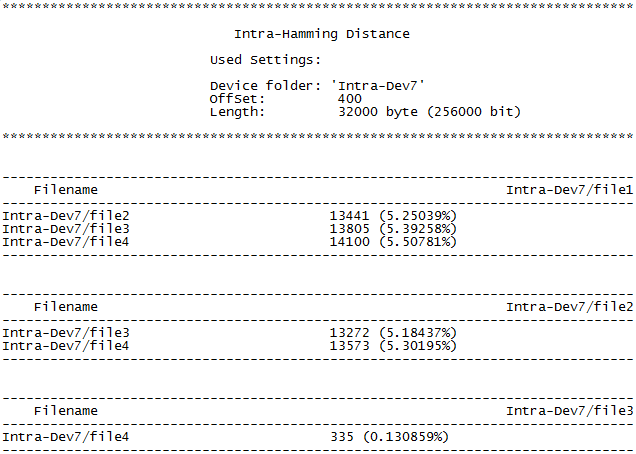
\includegraphics[width=0.9\textwidth]{images/4_intra_compact.png}}
\caption{Visualization of the \emph{compact} output style format.}
\label{img:4_intra_compact}
\end{figure}

\begin{figure}
\centering
\fbox{ 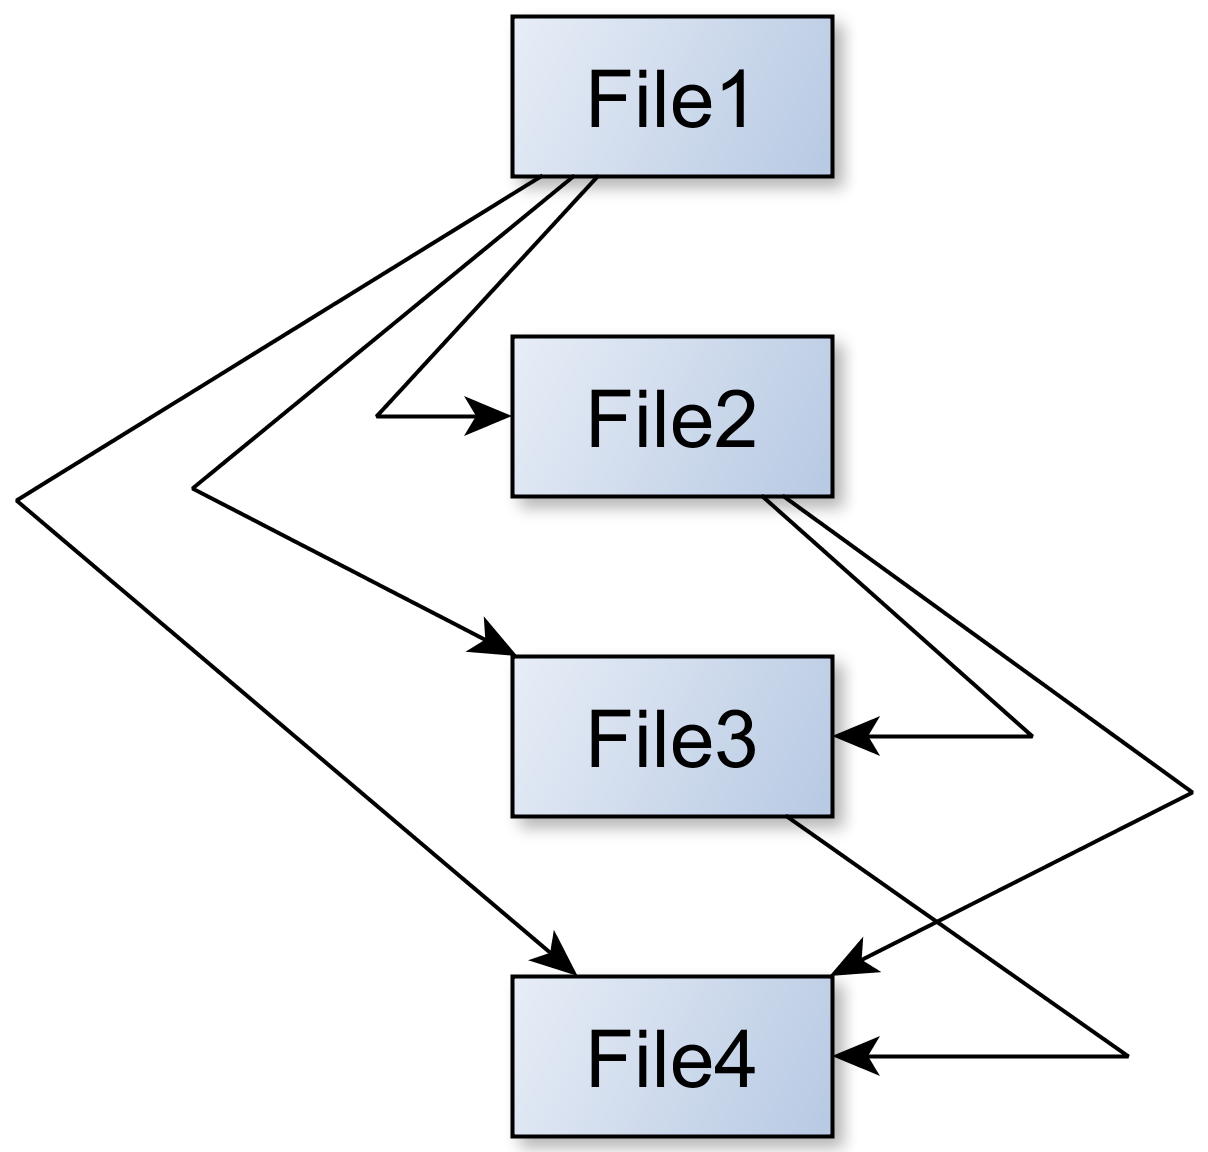
\includegraphics[width=0.4\textwidth]{images/Intra.png}}
\caption{Exemplary illustration of the working principle of the \emph{compact} mode, for the intra-Hamming distance.}
\label{img:4_intra_WP}
\end{figure}

A sample output file with compact style format is shown in Figure \ref{img:4_intra_compact} that evaluates the PUF instance from a single directory using Intra Hamming Distance metric, it also appends the fractional distance information to the file. It consists of a header with general information that shows the configuration (like offsets, device folder etc.) that was used for evaluation and three tables. In the upper right corner of each table the utilized input file is shown and on the left side of the table
the files, that are compared to the selected input file, are displayed. The Hamming Distance and Fractional Hamming Distance, seperated by a tab length are printed in the center (right) of each table. The
\emph{minimal} output style strips off all the path and filename info and only saves the Hamming Distance values seperated by spaces, this type of file format can be used by another metric of the toolkit called Median and Average [seb thesis section median] calculation which accepts only files containing plain numbers seperated with space. The \emph{View} option can be used to look at the output/result file.\\

\subsection{Inter Hamming Distance}
Contrary to the comparisons between PUF responses from the same device, Inter Hamming distance evaluates responses from different PUF instance. The co-relation is again based on the same metric Hamming Distance. In this case the toolkit can simulatneously compare from 2 to 99 PUF instances. All the PUF responses from a specific instance are arranged in a single directory so that means the toolkit can take input paths between 2 and 99 to evaluate different PUF devices. The output
style in addition to compact and minimal has a \emph{detailed} as an alternative. The compact and minimal style formats are same as Intra Hamming Distance, but the detailed style differs from the compact style that it does not implicitly ignores the duplicate symmetric comparisons and therefore maps out all the permutations and combinations between files of different folders. It should be noted that Inter Hamming Distance metric does not compare PUF responses in the same directory. So
in detailed mode, the first directory all the responses are compared to all the PUF responses from the remaining 3 to 99, then all files in second folder are compared to all the files in all the other folders except its own, and so on. The Figure \ref{ } shows a sample input with 3 input paths, for compact mode we need to ignore the duplicate comparisons so we take the following approach:
\begin{itemize}
	\item store all the filenames and their corresponding paths from all but last folder in list1.
	\item store all the filenames and their corresponding paths from all but first folder in list2.
	\item iterate over list1 (iteration 1-4) and compare the list1 objects with all entries of list2.
	\item remove the second folder objects from list2.
	\item iterate over list1 (iteration 5-7) and compare the list1 objects with all files of list2.
\end{itemize}

This process is summarized in Figure \ref{ } for three folder input and is generalized for more inputs. We emphasize on the inner workings of the modes because the exact same techniques are used for Jaccardi's index that will be discussed later in this chapter.\\

\emph{Menu Modifications:} In contrast to the original toolkit where Intra and Inter Hamming Distance were seperated in their own sub-menus, the new changes merges both of them under Hamming Distance Menu. Seeing as it is relevant to combine them if they use the same underlying metric, on the other hand the Hamming Weight menu item was untouched since it takes only one PUF response file as an input and gives out its hamming weight and there is no evaluation between two or
more files.\\


\section{Fuzzy extractor}
As discussed in section \ref{ } the PUF based secure key storage uses Fuzzy Extractor technique that is divided in three phases \emph{(i)Pre-evaluation}, \emph{(ii) Enrollment} and \emph{(iii) Reconstruction}. We discuss only the later two phases, where these two phases follow a seperate implementation of the respective dedicated functionalities, according to [seb 56]. The enrollment phase employs PUF BCH encoder which will be discussed first followed by the Reconstruction phase, that is
realized by the PUF BCH Decoder implementation. We will not go into the details of the actual implementation of the encoder and decoder since thay are already well documented in [Master theses sebastian], but rather explain the changes made to integrate these functionalities in the PUF toolkit.\\

The concept of fuzzy extractor in combination with BCH coding with linear repetition code and majority vote is depicted in Figures \ref{4_BCH_concept}, \ref{4_LR_HD} and \ref{4_MV_codewords}.\pagebreak

\begin{figure}[h]
\centering
\fbox{ 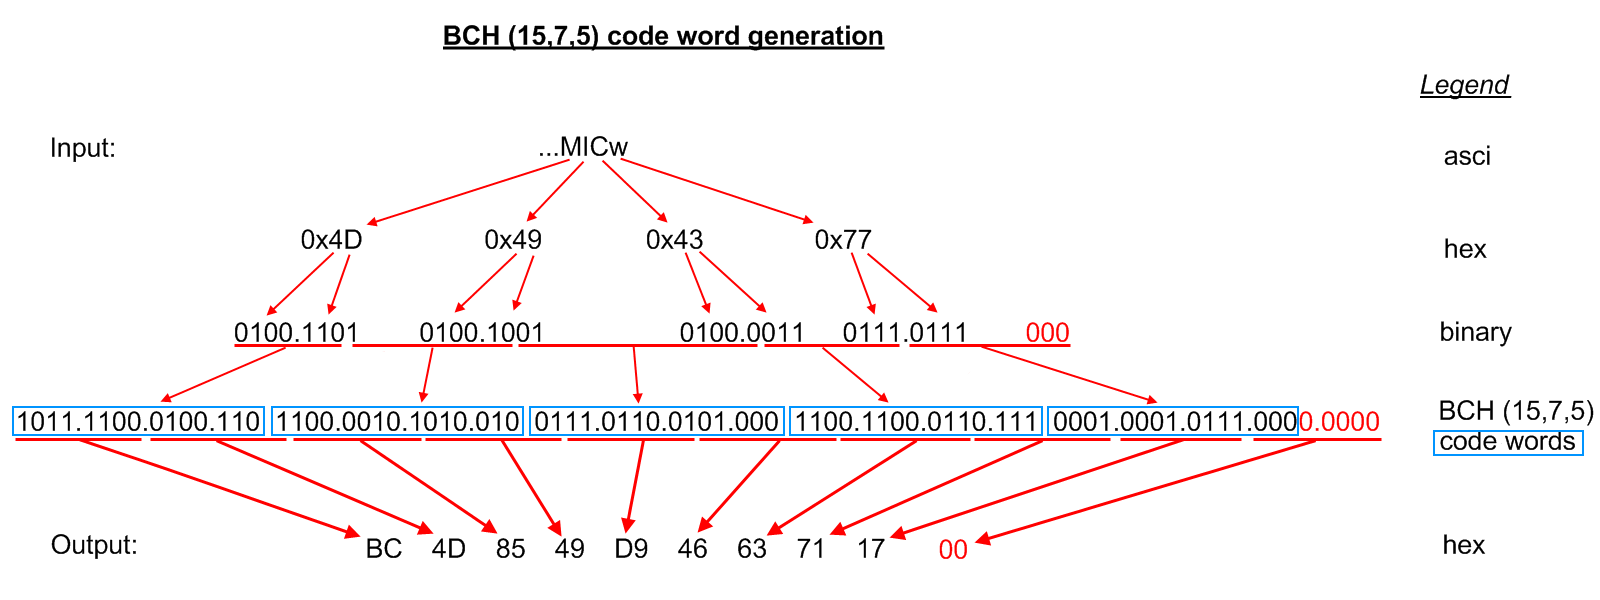
\includegraphics[width=0.97\textwidth]{images/BCHconcept.png}}
\caption{Exemplary code word generation with a BCH (15,7,5) code, based on \cite{10}.}
\label{img:4_BCH_concept}
\end{figure}

\begin{figure}[h]
\centering
\fbox{ 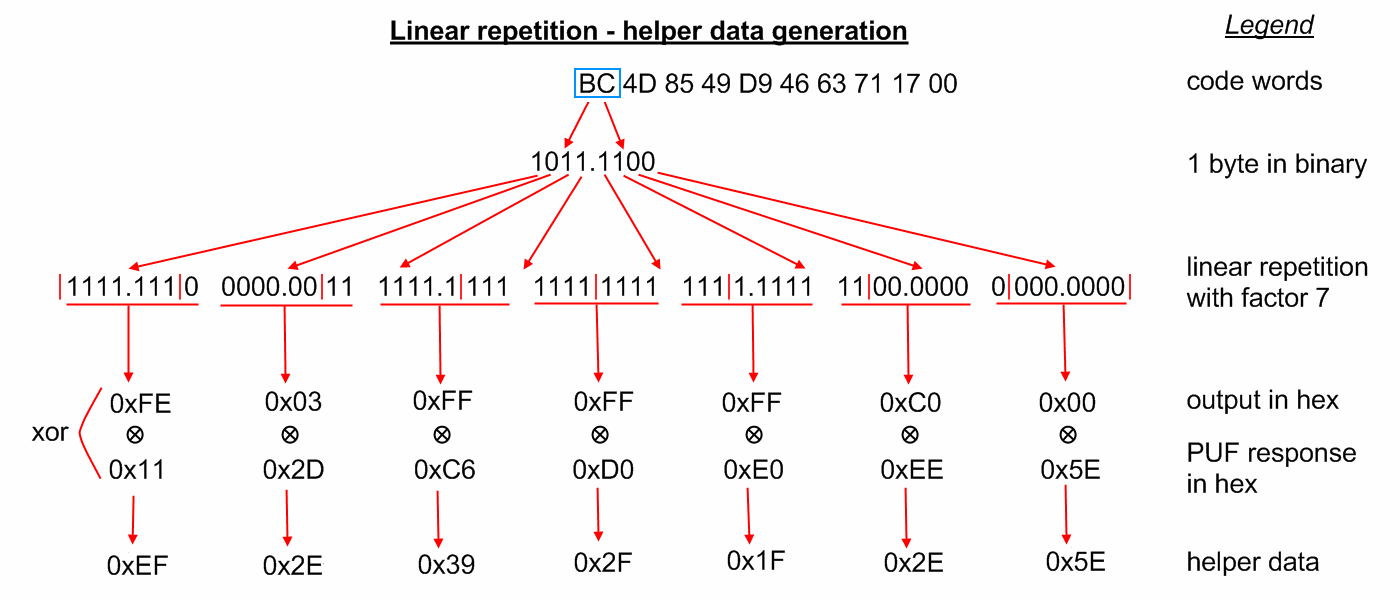
\includegraphics[width=0.97\textwidth]{images/LRhd.png}}
\caption{Exemplary helper data generation with a linear repetition code and factor 7, based on \cite{10}.}
\label{img:4_LR_HD}
\end{figure}

\begin{figure}[h]
\centering
\fbox{ 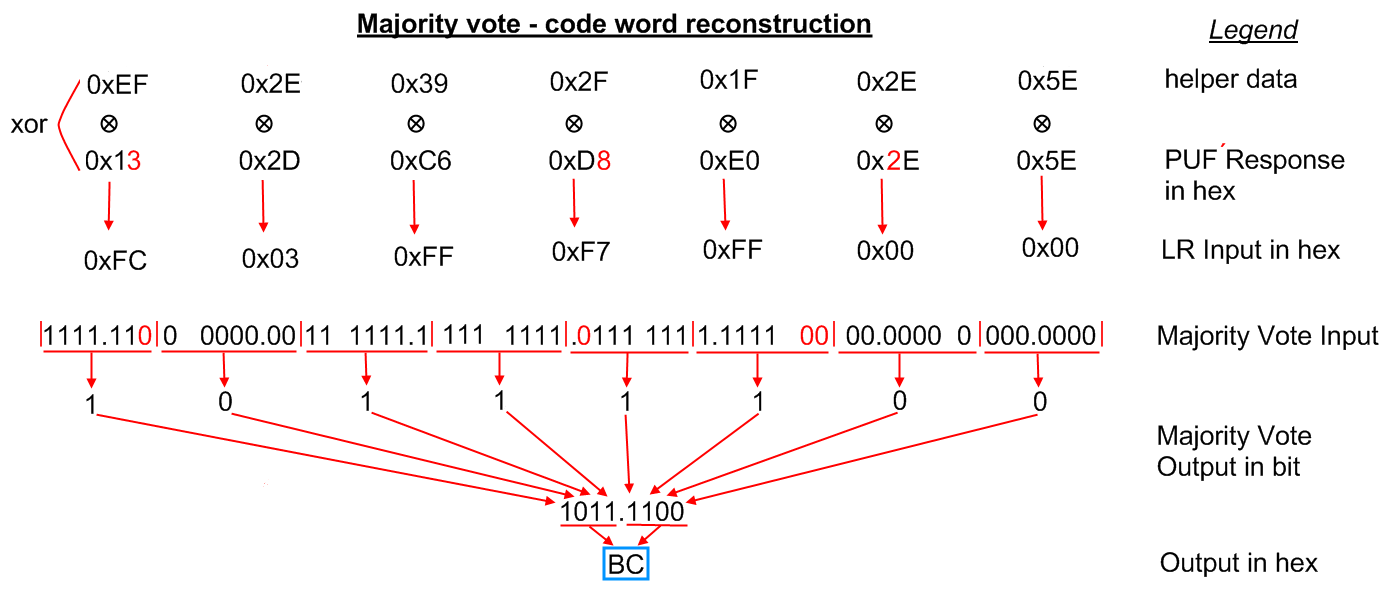
\includegraphics[width=0.97\textwidth]{images/MVrecon.png}}
\caption{Exemplary code word reconstruction with the majority vote and factor 7, based on \cite{10}.}
\label{img:4_MV_codewords}
\end{figure}

\subsection{PUF BCH Encoder}
We first briefly mention the implementation algorithm used in the BCH encoding of the data, after that the user interface is illustrated followed by a Entity relation diagram that shows major functions of the encoder. We present the changes as a subsection named integration changes and we conclude with steps taken to verify the integrated BCH encoder.\\

The BCH encoding implementation is taken from \emph{Morelos-Zaragozas Encoder/Decoder} for binary BCH codes in C [seb 43]. This algorithm uses systematic encoding to encode the message, hence the encoded codewords contain initial message in it, which is stripped from the codeword to get the helper data, using the BCH(n,k,d) (refer section \ref{bch section}) the codewords are combined in groups of \emph{length k} and extra 0s are added to complete the last set as shown in Figure \ref{ }. In the
second part of the enrollment of the fuzzy extractor the LR code is applied to the generated codeword, based on the user input the bits are repeated either 7 or 15 times, the Figure \ref{ } shows this LR process with factor 7. It was noted that there were some limitations to the original algorithm and the encoding only works for small values of $m$, after code review and research the error states were removed and/or documented.\\

Due to above mentioned limitations, the correct combination of BCH encoding and linear repetition code requires correct handling of the bounds. The length of the secret key in bits is denoted by $N$, to process the entire file with BCH (n,k,d) code we need \emph{len} iterations of encoding, this is defined in equation \ref{4:BCH_len}.

\begin{itemize}
	\item For an input data of length \emph{N} (bits) and a BCH ($n$,$k$,$d$) code, a ‘\emph{len}’ number of BCH encoding iterations have to be performed to process the complete input file [Master thesis seb]:
\begin{equation}
	len =\Bigg\lceil\dfrac{N}{k}\Bigg\rceil
	\label{4:BCH_len}
\end{equation}

\item For a BCH ($n$,$k$,$d$) code that requires ‘\emph{len}’ BCH encoding iterations to process the complete input file, the result of the linear repetition code has a length of ‘\emph{LengthAfterLR}’ with respect to the chosen linear repetition factor ‘\emph{LRfactor}’ (7 or 15) [Master Thesis Sebastian]:
\begin{equation}
	LengthAfterLR = \Bigg\lceil\Bigg(\dfrac{\Bigg(\dfrac{len}{k} * n\Bigg)}{8}\Bigg)\Bigg\rceil * LRfactor
\label{4:BCH_LR_len}
\end{equation}
\end{itemize}

The User interface for the BCH sub menu is shown in Figure \ref{ }. The first option is to set the BCH mode in which the user is required to input the codelength $n$ i.e. derived from $m$ such that $(2^{m-1} - 1) < length <= (2^m - 1)$, after that it is also mandatory to enter the desired correction capability $t$ of the BCH (n,k,d) code that in turn will determine the paramter $d$ of the code from the formula \ref{ }.
These values must be consistent with the equations \ref{4:BCH_len} and \ref{4:BCH_LR_len} or else the decoding of the secret key will not be successful. The second option chooses the LR factor as 7 or 15, the third is the familiar offsets selection for the PUF response that will also determine the actual length of the PUF response used to generate the helper data. After this the user must also input the key he/she wants to securely store and the name of the PUF
response file, finally the output filename for helperdata must be provided to be saved on permanent storage and to be used in the later reconstruction phase of the fuzzy extraction. These discussed inputs are all mandatory in the BCH menu and only then we can use option seven to process and generate the helper data or else the toolkit throws appropriate error messages to the user about missing parameters.\\

We show the functions of the BCH encoder arranged in modules that are related to each other via Figure \ref{img:bchenc_fns}

\begin{figure}
\centering
\fbox{ \includegraphics[width=0.9\textwidth]{images/bch_encoder_functions.pdf}}
\caption{Dependencies of the BCH Encoder Modules}
\label{img:bchenc_fns}
\end{figure}

The data structure \emph{Item} that was discussed in Hamming Distance contains relevant data members related to BCH encoder, which are summarized in the table \ref{tab:4_BCH_DEC_item_type_limits}

\begin{table}[!ht]
\begin{center}
\begin{tabular}{lll}
\toprule
\multicolumn{1}{l}{\textbf{Name}} & \multicolumn{1}{c}{\textbf{Type}} & \multicolumn{1}{c}{\textbf{Description}}\\
\midrule
\hline

\emph{offset\_begin} & long & \multicolumn{1}{l}{\begin{tabular}[l]{@{}l@{}}Defines the starting point in a binary file (bytes to skip from beginning) \end{tabular}}\\

\emph{offset\_end} & long & \multicolumn{1}{l}{\begin{tabular}[l]{@{}l@{}}Defines the ending point in a binary file (bytes to skip from end) \end{tabular}}\\

\emph{input\_HD\_name} &  char [102] & \multicolumn{1}{l}{\begin{tabular}[l]{@{}l@{}}Char array for 102 symbols, to define the input helper data file \end{tabular}}\\

\emph{input\_PUF\_name} & char [102] & \multicolumn{1}{l}{\begin{tabular}[l]{@{}l@{}}Char array for 102 symbols, to define the input PUF file \end{tabular}}\\

\emph{output\_Key\_name} & char [102] & \multicolumn{1}{l}{\begin{tabular}[l]{@{}l@{}}Char array for 102 symbols, to define the output key file \end{tabular}}\\

\emph{BCHmode} & char [25] & \multicolumn{1}{l}{\begin{tabular}[l]{@{}l@{}}Char array for 25 symbols, to define the BCH mode \end{tabular}}\\

\emph{LR} & int & \multicolumn{1}{l}{\begin{tabular}[l]{@{}l@{}}Definition of the utilized linear repetition factor \end{tabular}}\\

\emph{result} & char [52] & \multicolumn{1}{l}{\begin{tabular}[l]{@{}l@{}}Char array for 52 symbols, to provide feedback \end{tabular}}\\
\hline
\addlinespace
\bottomrule
\end{tabular}
\end{center}

\caption{Names and types of data memebers of the data structure \emph{Item} for the \emph{PUF BCH Decoder} and a brief description .}
\label{tab:4_BCH_DEC_item_type_limits}
\end{table}

\subsubsection{Integration changes}
Initially the BCH Menu item was defined in the toolkit module to be called by the main menu, after that support for Offset from beginning and end, depicted in table \ref{tab:4_BCH_DEC_item_type_limits}, was made available similar to Hamming Distance menu. Since the ``Calculation module'' functions of the BCH encoder are all called internally without any dependence on the user, so they were unified with the original PUF Toolkit Calculation module without much hindrance.
The ``Settings module'' was merged to the toolkit with \emph{DefineFilename\_BCH} was renamed to avoid function name conflict with \emph{DefineFilename} of the toolkit, the former is dedicated to process the input PUF filename, output helperdata file and input secret key of the BCH encoder. The ``File and View modules'' were straightforward to unify with the toolkit, special care was taken to add the BCH global variables and global vectors to the toolkit. Changes in the ``View
module'' were dominated by the \emph{ErrorMessages} routine, which informs the user about the incorrect input and error states and the ways to recover from them. Major challenges faced during the integration were the same name functions as in the orignal toolkit that resulted in linking errors, they were resolved by renaming them appropriately for BCH encoder and all the declarations of the resulting functions were unified in the header files of the respective modules.\\

\subsubsection{Verification}
The correctness after merging the BCH encoder was authenticated via exhaustive run through all the test cases. In addition to that a final verification of the entire implementation was done. While doing the verification following main points were given priority:

\begin{itemize}
	\item Correctness of each module verified through utilization of test cases.
	\item All the possible menu options were checked and reviewed for their expected functionality
	\item Wrong inputs and incorrect state handling was also tested to make sure that the toolkit accepts only legitimate inputs and display appropriate error messages to rectify the error.
	\item Unusual workflows were inspected to assess their impact on Encoder functionality.
\end{itemize}
\pagebreak

\subsection{PUF BCH Decoder}


